\section{Scaling laws and Emergent Behavior}
\label{sec:scaling_laws}

% \mrinmaya{Maybe we should move this to the last chapter.}
% \mrinmaya{Can we motivate why studying this is helpful/important. What is the relevance of this?}

With the improved accuracy of pretrained language models, researchers noticed improvements in performance with increasing model size. 

% \mrinmaya{Should we say how the experiment was conducted? Or too complicated? SD: I think the details can be complicated and we can point them to the paper. There's a lot going on in this and it's very empirical. I think we can just add the eqns. SD:Simplified and added the eqns}
\citet{kaplan2020scaling} demonstrate that the test-loss of an autoregressive transformer exhibits a power-law relationship when the model's performance is constrained by only one of three factors: the number of non-embedding parameters $(N)$, the size of the dataset $(D)$, or the compute budget allocated optimally $(C_{min})$.
%\mrinmaya{Maybe we can write down the function form from the paper.}
They analyze the relationship between language modeling loss and these factors, with a focus on the Transformer architecture. The broad range of performance levels in language tasks enables us to examine trends across more than seven orders of magnitude in scale.

The authors identify precise power-law scaling patterns for performance in relation to training time, context length, dataset size, model size, and computational resources.
% show that the test-loss of an autoregressive transformer follows the power-law when performance is limited by only either the number of non-embedding parameters $N$, the dataset size $D$, or the optimally allocated compute budget $C_{min}$.
% They also show that these relations hold across eight orders of magnitude in $C_{min}$, six orders of magnitude in $N$, and over two
% orders of magnitude in $D$ and they depend very weakly on model shape and other Transformer hyperparameters
% (depth, width, number of self-attention heads), with other properties of similarity associated with the training set.



\paragraph{Summary of Scaling Laws.}

The test loss of a Transformer trained to autoregressively model language can be predicted using a power-law  when performance is limited by only either the number of non-embedding parameters $N$, the dataset size $D$, or the optimally allocated compute budget $C_{\rm min}$ (see \Cref{fig:scaling_1}):
% fig:BasicPowerLaws
\begin{enumerate}
\setlength\itemsep{0.5em}
\item For models with a limited number of parameters, trained to convergence on sufficiently large datasets:
$L(N) = \left(N_{\mathrm{c}}/N\right)^{\alpha_N};~~ \alpha_N \sim 0.076, \quad N_{\mathrm{c}} \sim 8.8 \times 10^{13}~\text{(non-embedding parameters)} \label{eq:crit_n}$
\item For large models trained with a limited dataset with early stopping:
$L(D) = \left(D_{\mathrm{c}}/D\right)^{\alpha_D};~~ \alpha_D \sim 0.095, \quad D_{\mathrm{c}} \sim 5.4 \times 10^{13}~\text{(tokens)} \label{eq:crit_d}$
\item When training with a limited amount of compute, a sufficiently large dataset, an optimally-sized model, and a sufficiently small batch size:
$L(C_{\rm min}) = \left(C_{\mathrm{c}}^{\rm min} / C_{\rm min}\right)^{\alpha_C^{\rm min}};~~ \alpha_C^{\rm min} \sim 0.050, \quad C_{\mathrm{c}}^{\rm min} \sim 3.1 \times 10^{8}~\text{(PF-days)} \label{eq:crit_c}$
\end{enumerate}

These relations hold across eight orders of magnitude in $C_{\rm min}$, six orders of magnitude in $N$, and over two orders of magnitude in $D$.  They depend very weakly on model shape and other Transformer hyperparameters (depth, width, number of self-attention heads).   The power laws $\alpha_{\rm N}, \alpha_{\rm D}, \alpha_{C}^{\rm min}$ specify the degree of performance improvement expected as we scale up $N$, $D$, or $C_{\rm min}$; for example, doubling the number of parameters yields a loss that is smaller by a factor $2^{-\alpha_N}=0.95$. The precise numerical values of $N_{\mathrm{c}}, C_{\rm c}^{\rm min},$ and $D_{\mathrm{c}}$ depend on the vocabulary size and tokenization and hence do not have a fundamental meaning.  



% \textbf{Performance depends strongly on scale, weakly on model shape:} Model performance is primarily influenced by scale, which consists of three factors: the number of model parameters $N$ (excluding embeddings), the size of the dataset $D$, and the amount of compute $C$ used for training. 
% Within reasonable limits,
% performance depends very weakly on other architectural hyperparameters such as depth versus width. 

% \textbf{Smooth power laws}: 
% Performance exhibits a power-law relationship with each of the three scale factors $N$, $D$, and $C$ when not restricted by the other two, with trends spanning over six orders of magnitude.
% % We observe no signs of deviation from these trends on the upper end, though performance
% % must flatten out eventually before reaching zero loss. \mrinmaya{Cant understand this sentence. We can remove.}

% \textbf{Universality of overfitting}: 
% Performance predictably improves as long as we scale up $N$ and $D$ in tandem, but enters a regime of diminishing returns if either $N$ or $D$ is held fixed while the other increases. 
% The performance penalty depends predictably on the ratio $N^{0.74}/D$, meaning that every time we increase the
% model size $8x$, we only need to increase the data by roughly $5x$ to avoid a penalty. 
% \mrinmaya{Can we say how the experiment was conducted?}


% \textbf{Universality of training:} 
% Training curves follow predictable power-laws whose parameters are roughly independent of the model size. 
% By extrapolating the early part of a training curve, we can roughly predict the loss that would be achieved if we trained for much longer. 

% \textbf{Transfer improves with test performance:} 
% \mrinmaya{Cant understand some of this. What is the offset. We dont need to copy paste from the paper. We can keep the main messages and just summarize in our own words. No need to also talk about everything in the paper}
% When we evaluate models on text with a different distribution than they were trained on, the results are strongly correlated to those on the training validation set with a roughly constant offset in the loss – in other words, transfer to a different distribution incurs a constant penalty but otherwise improves roughly in line with performance on the training set. 
% \\
% \textbf{Sample efficiency:} Large models are more sample-efficient than small models, reaching the same level of
% performance with fewer optimization steps and using fewer data points.

% \textbf{Convergence is inefficient:} When working within a fixed compute budget $C$ but without any other restrictions on the model size $N$ or available data $D$, we attain optimal performance by training very large models and stopping significantly short of convergence. 
% Maximally compute-efficient training would therefore be far more sample efficient than one might expect based on training small models to convergence, with data requirements growing very slowly as $D \sim C^{0.27}$ with training compute.

% \textbf{Optimal batch size:} The ideal batch size for training these models is roughly a power of the loss only,
% and continues to be determinable by measuring the gradient noise scale; it is roughly $1-2$ million
% tokens at convergence for the largest models we can train. 

% \mrinmaya{I thought this was test loss.}
% Their empirical results showing the training loss change with respect to the number of non-embedding parameters, the dataset size, and the compute budget are described in Figure \ref{fig:scaling_1} and \ref{fig:scaling_2}.

Scaling a model can give rise to some emergent abilities.
\cite{wei2022emergent} describe an emergent ability as 
\begin{quote}
\textit{    An ability is emergent if it is not present in smaller models but is present in larger models.
}
\end{quote}


\cite{wei2022emergent} compare how models of varying sizes perform on various tasks and show that abilities to perform some tasks emerge in language models after a certain scale.
Figure \ref{fig:emergent_1} and \ref{fig:emergent_2} show how language models that are trained above a certain number of FLOPS exhibit increased performance on certain tasks.


\begin{figure*}[htbp]
  \centering
    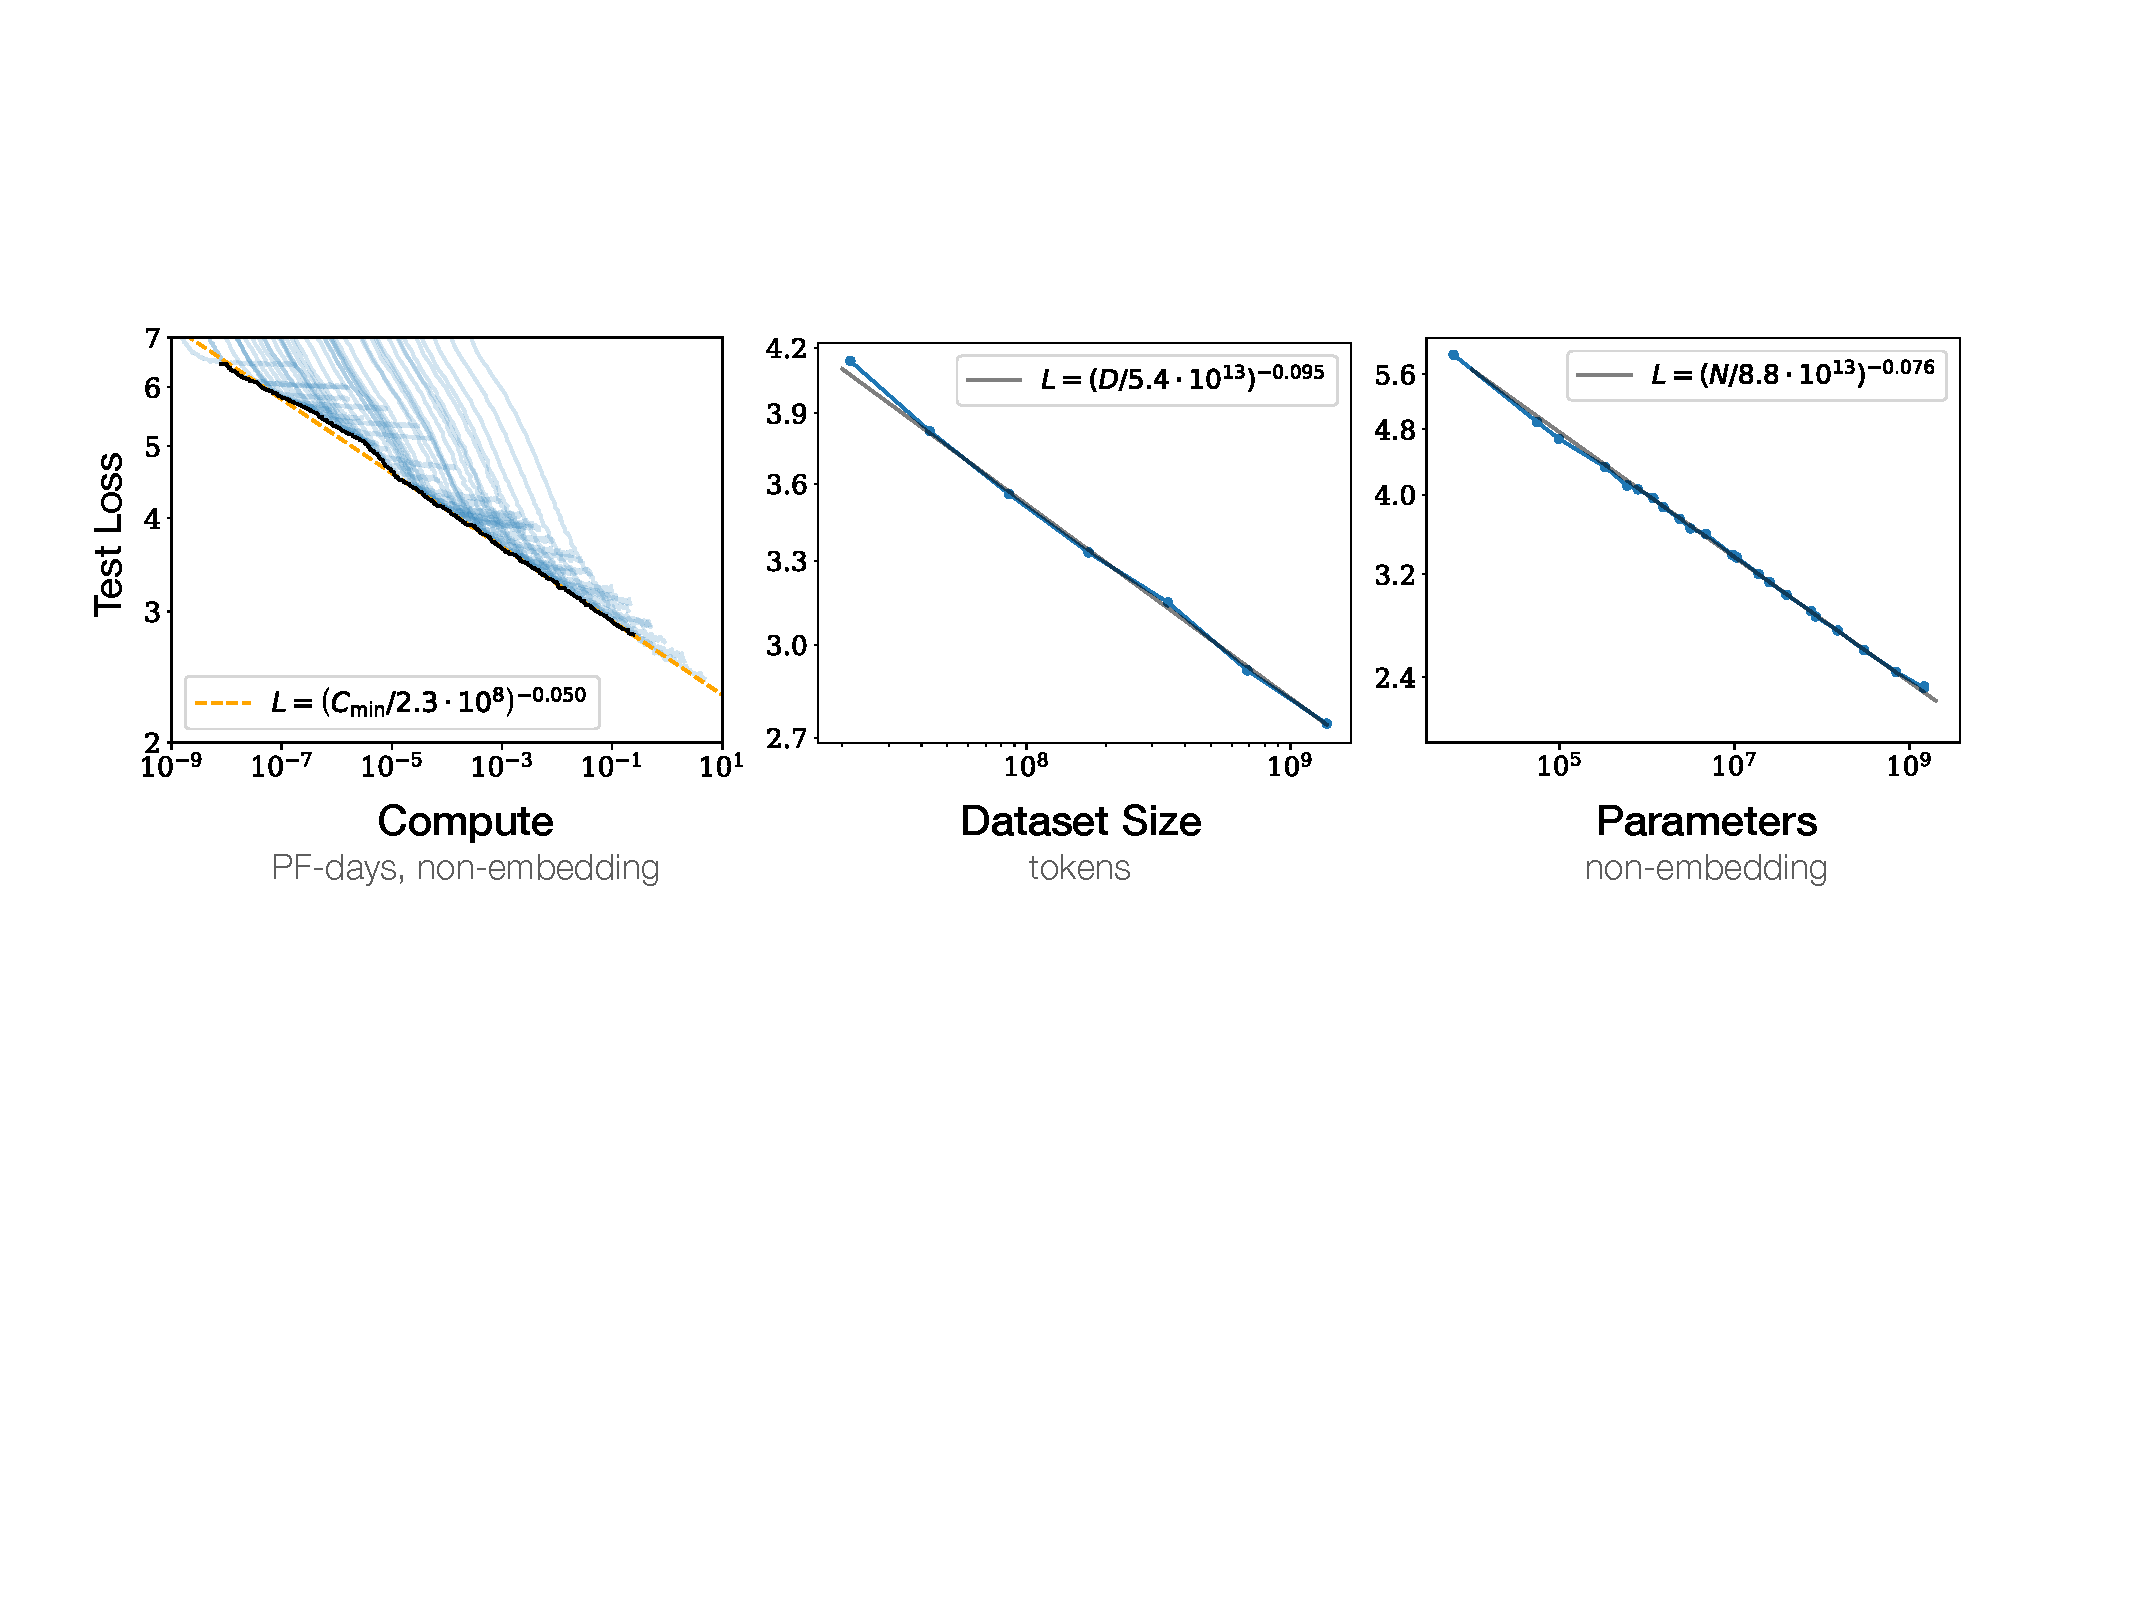
\includegraphics[width=\textwidth]{figures/transfer_learning/SimplePowerLaws.pdf}
  \caption{Language modeling performance improves smoothly as we increase the model size, datasetset
size, and amount of compute used for training. For optimal performance all three factors must be scaled
up in tandem. }
  \label{fig:scaling_1}
  \vspace{-3mm}
\end{figure*}


\begin{figure*}[htbp]
  \centering
    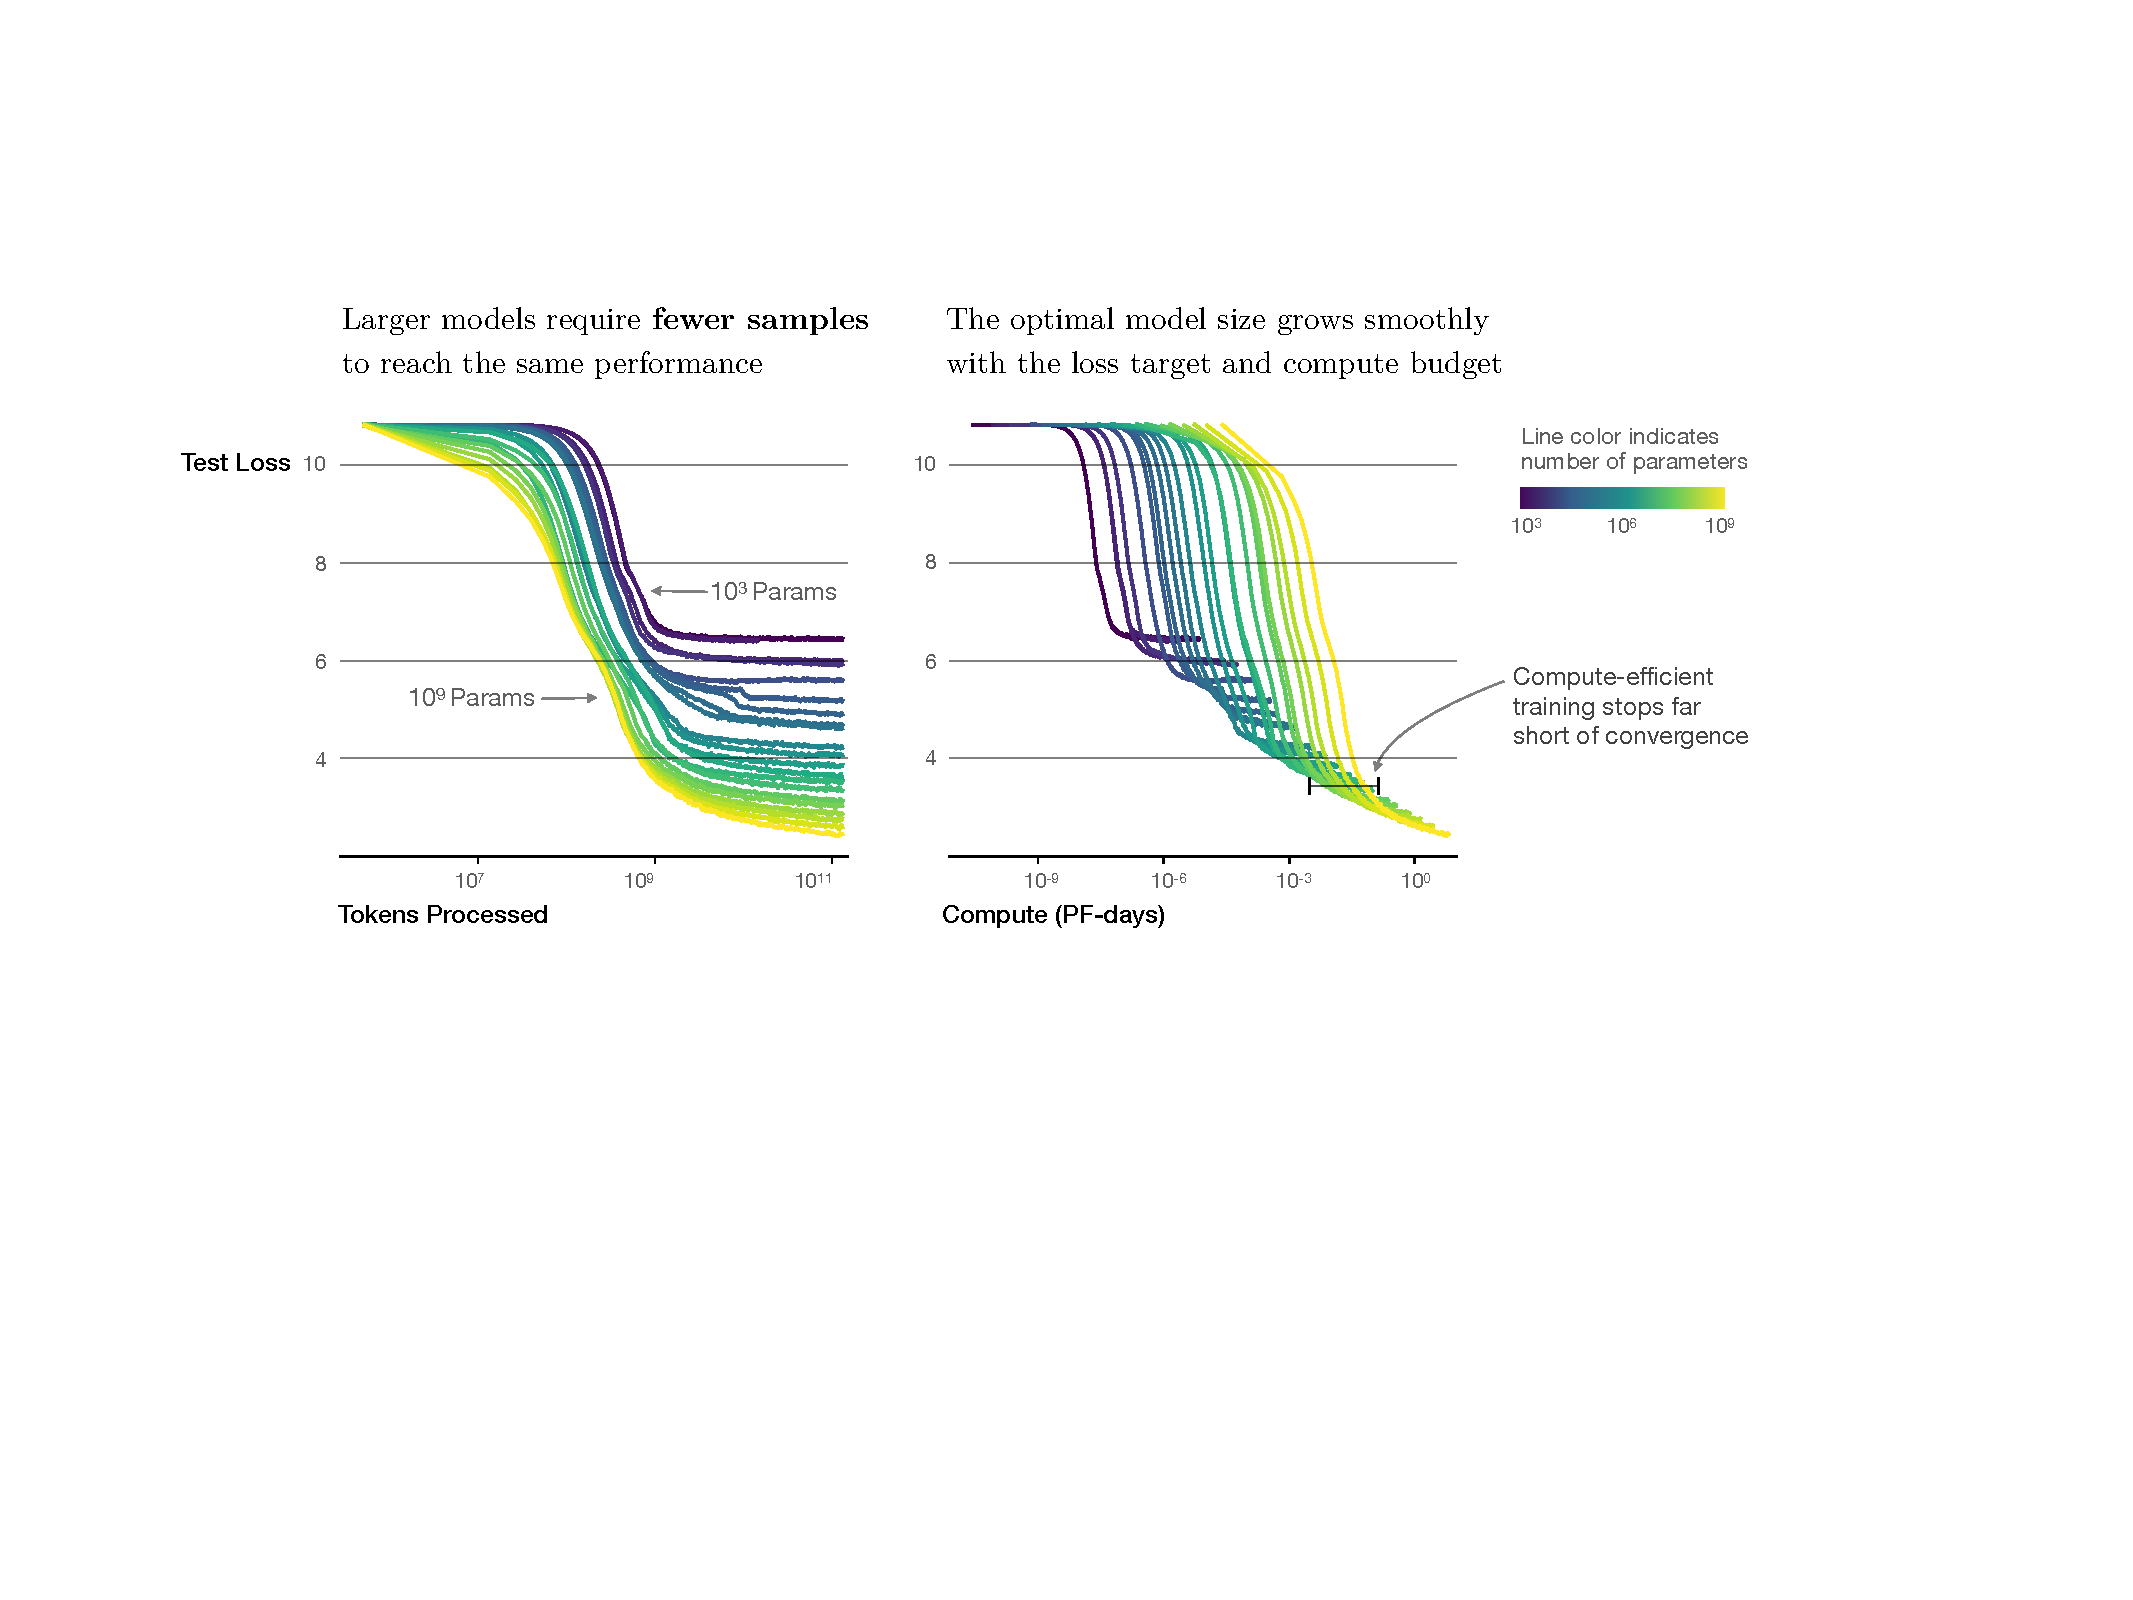
\includegraphics[width=\textwidth]{figures/transfer_learning/EfficiencyIllustration.pdf}
  \caption{Language model training runs, with models ranging in size from $10^3$
to $10^9$
parameters (excluding embeddings).}
  \label{fig:scaling_2}
  \vspace{-3mm}
\end{figure*}


\begin{figure*}[ht]
    \begin{centering}
    \scalebox{0.7}{
    \begin{tikzpicture}
        \pgfplotsset{footnotesize,samples=10}
        \begin{groupplot}[
            group style = {group size = 4 by 1, horizontal sep = 42pt},
            width = 4.2cm, 
            height = 5cm]
            \nextgroupplot[
                align = center,
                title = {\textbf{(A) Mod.~arithmetic}},
                legend style={at={(-0.12,1.4)},anchor=south},
                xmode=log,
                xmin=3e17, xmax=3e24,
                ymin=-4, ymax=52,
                xtick={1e18,1e20,1e22,1e24},
                axis x line*=bottom,
                axis y line*=left,
                ylabel={Accuracy (\%)},
                ytick={0, 10, 20, 30, 40, 50},
                grid style=dashed,
                x label style={at={(axis description cs:0.5,-0.15)},anchor=north},
                y label style={at={(axis description cs:-0.16,0.5)},anchor=south},
                xtick pos=bottom,
                ytick pos=left,
                ]
                \addplot[
                    color=frenchblue,
                    mark=*,
                    mark size=1.5pt,
                    line width=1pt,
                    ]
                    coordinates {
                    (3.3e18,  0.3)
                    (3.16e19, 0.3)
                    (8.9e19,  0.2)
                    (1.4e20,  0.1)
                    (4.2e20,  0.3)
                    (4.08e20, 0.4)
                    (9.1e20,  0.4)
                    (1.72e21,      0.6)
                    (2.86e21,      0.69)
                    (6.78e21,    0.78)
                    (2.3e22,     0.9)
                    (1.2e23,     7.6)
                    (5.54e23,  15.7)
                    };
                \addplot[
                    color=frenchlilac,
                    mark=square*,
                    mark size=1.3pt,
                    line width=1pt,
                    ]
                    coordinates {
                    (2.25e20 , 0.6)
                    (6.41e20 , 0.6)
                    (1.37e21 , 0.7)
                    (2.38e21 , 0.5)
                    (4.77e21 , 0.6)
                    (1.20e22 , 1.6)
                    (2.31e22 , 8.7)
                    (3.14e23 , 33)
                    };
                \addplot[
                    color=frenchrose,
                    mark=square,
                    no markers,
                    dashed,
                    line width=1.3pt,
                    ]
                    coordinates {
                    (1, 0)
                    (1e25, 0)
                    };
            \nextgroupplot[
                align = center,
                title = {\textbf{(B) IPA transliterate}},
                legend style={at={(-0.12,1.4)},anchor=south},
                xmode=log,
                xmin=3e17, xmax=3e24,
                ymin=-4, ymax=52,
                xtick={1e18,1e20,1e22,1e24},
                axis x line*=bottom,
                axis y line*=left,
                ytick={0, 10, 20, 30, 40, 50},
                ylabel={BLEU (\%)},
                grid style=dashed,
                x label style={at={(axis description cs:0.5,-0.15)},anchor=north},
                y label style={at={(axis description cs:-0.16,0.5)},anchor=south},
                xtick pos=bottom,
                ytick pos=left,
                ]
                \addplot[
                    color=frenchblue,
                    mark=*,
                    mark size=1.5pt,
                    line width=1pt,
                    ]
                    coordinates {
                    (3.3e18,  0.12)
                    (3.2e19,  0.12)
                    (8.9e19,  0.26)
                    (1.4e20,  0.31)
                    (4.2e20,  0.14)
                    (4.1e20,  0.37)
                    (9.1e20,      0.54)
                    (1.7e21,      0.61)
                    (2.96e21,      0.45)
                    (6.8e21,      0.77)
                    (2.3e22,     0.99)
                    (1.2e23,     15.2)
                    (5.4e23,    22.5)
                    };
                \addplot[
                    color=frenchlilac,
                    mark=square*,
                    mark size=1.3pt,
                    line width=1pt,
                    ]
                    coordinates {
                    (2.25e20 , 0.59)
                    (6.41e20 , 0.17)
                    (1.37e21 , 0.25)
                    (2.38e21 , 0.85)
                    (4.77e21 , 2.46)
                    (1.20e22 , 3.8)
                    (2.31e22 , 4.83)
                    (3.14e23 , 22.82)
                    };
                \addplot[
                    color=frenchrose,
                    mark=square,
                    no markers,
                    dashed,
                    line width=1.3pt,
                    ]
                    coordinates {
                    (1, 0)
                    (1e25, 0)
                    };
            \nextgroupplot[
                align = center,
                title = {\textbf{(C) Word unscramble}},
                legend style={at={(-0.2,1.25)},anchor=south,draw=none
                ,/tikz/column 2/.style={column sep=8pt,}
                ,/tikz/column 4/.style={column sep=8pt,}
                ,/tikz/column 6/.style={column sep=8pt,}
                ,/tikz/column 8/.style={column sep=8pt,}
                ,/tikz/column 10/.style={column sep=8pt,}
                ,},
                legend columns=-1,
                xmode=log,
                xmin=3e17, xmax=3e24,
                ymin=-4, ymax=52,
                xtick={1e18,1e20,1e22,1e24},
                axis x line*=bottom,
                axis y line*=left,
                ytick={0, 10, 20, 30, 40, 50},
                ylabel={Exact match (\%)},
                grid style=dashed,
                x label style={at={(axis description cs:0.5,-0.15)},anchor=north},
                y label style={at={(axis description cs:-0.16,0.5)},anchor=south},
                xtick pos=bottom,
                ytick pos=left,
                ]
                \addplot[
                    color=frenchblue,
                    mark=*,
                    mark size=1.5pt,
                    line width=1pt,
                    ]
                    coordinates {
                    (3.3e18,  0.87)
                    (3.2e19,  0)
                    (8.9e19,  0.0)
                    (1.4e20,  0.0)
                    (4.2e20,  0.3)
                    (4.1e20,  0.3)
                    (9.1e20,      0.7)
                    (1.7e21,      1)
                    (2.96e21,     1.2)
                    (6.8e21,      2.3)
                    (2.3e22,     1.9)
                    (1.2e23,     10.7)
                    (5.4e23,    12.3)
                    };
                    \addlegendentry{LaMDA}
                \addplot[
                    color=frenchlilac,
                    mark=square*,
                    mark size=1.3pt,
                    line width=1pt,
                    ]
                    coordinates {
                    (1e25, 100)
                    };
                    \addlegendentry{GPT-3}
                \addplot[
                    color=jweigreen,
                    mark=diamond*,
                    mark size=2.3pt,
                    line width=1pt,
                    ]
                    coordinates {
                    (1e25, 100)
                    };
                    \addlegendentry{Gopher}
                \addplot[
                    color=frenchbeige,
                    mark=triangle*,
                    mark size=2.5pt,
                    line width=1pt,
                    ]
                    coordinates {
                    (1e25, 100)
                    };
                    \addlegendentry{Chinchilla}
                \addplot[
                    color=frenchblue,
                    mark=pentagon*,
                    mark size=3pt,
                    line width=1pt,
                    ]
                    coordinates {
                    (1e25, 100)
                    };
                    \addlegendentry{PaLM}
                \addplot[
                    color=frenchrose,
                    mark=square,
                    no markers,
                    dashed,
                    line width=1.3pt,
                    ]
                    coordinates {
                    (1, 0)
                    (1e25, 0)
                    };
                    \addlegendentry{Random}
            \nextgroupplot[
                align = center,
                title = {\textbf{(D) Persian QA}},
                legend style={at={(1,1.5)},anchor=east,draw=none},
                xmode=log,
                xmin=3e17, xmax=3e24,
                ymin=-4, ymax=52,
                xtick={1e18,1e20,1e22,1e24},
                axis x line*=bottom,
                axis y line*=left,
                ytick={0, 10, 20, 30, 40, 50},
                ylabel={Exact match (\%)},
                grid style=dashed,
                x label style={at={(axis description cs:0.5,-0.15)},anchor=north},
                y label style={at={(axis description cs:-0.16,0.5)},anchor=south},
                xtick pos=bottom,
                ytick pos=left,
                ]
                \addplot[
                    color=frenchblue,
                    mark=*,
                    mark size=1.5pt,
                    line width=1pt,
                    ]
                    coordinates {
                    (3.3e18, 25.9)
                    (3.2e19, 22.7)
                    (8.9e19, 23.6)
                    (1.4e20, 24.6)
                    (4.2e20, 24.2)
                    (4.1e20, 23.5)
                    (9.1e20, 24.1)
                    (1.7e21, 22.9)
                    (2.96e21, 25.1)
                    (6.8e21, 25.8)
                    (2.3e22, 23.7)
                    (5.4e23, 23.6)
                    };
                \addplot[
                    color=frenchlilac,
                    mark=square*,
                    mark size=1.3pt,
                    line width=1pt,
                    ]
                    coordinates {
                    (2.25e20 , 25)
                    (6.41e20 , 24.1)
                    (1.37e21 , 24.3)
                    (2.38e21 , 24.4)
                    (4.77e21 , 26)
                    (1.20e22 , 24.7)
                    (2.31e22 , 25)
                    (3.14e23 , 24.2)
                    };
                \addplot[
                    color=frenchblue,
                    mark=pentagon*,
                    mark size=3pt,
                    line width=1.3pt,
                    ]
                    coordinates {
                    (3.7e22,  24.4)
                    (2.9e23,  29.1)
                    (2.5e24, 45.3)
                    };
                \addplot[
                    color=frenchrose,
                    mark=square,
                    no markers,
                    dashed,
                    line width=1.3pt,
                    ]
                    coordinates {
                    (1, 25)
                    (1e25, 25)
                    };
        \end{groupplot}
    \end{tikzpicture}}
    \\ \vspace{6mm}
    \scalebox{0.7}{
    \begin{tikzpicture}
        \pgfplotsset{footnotesize,samples=10}
        \begin{groupplot}[
            group style = {group size = 4 by 1, horizontal sep = 42pt},
            width = 4.2cm, 
            height = 5cm]
            \nextgroupplot[
                align = center,
                title = {\textbf{(E) TruthfulQA}},
                legend style={at={(-0.12,1.4)},anchor=south},
                xmode=log,
                xmin=3e19, xmax=3e24,
                ymin=-4, ymax=72,
                xtick={1e20, 1e22, 1e24},
                axis x line*=bottom,
                axis y line*=left,
                ylabel={Accuracy (\%)},
                ytick={0, 10, 20, 30, 40, 50, 60, 70},
                grid style=dashed,
                x label style={at={(axis description cs:0.5,-0.18)},anchor=north,font=\normalsize},
                y label style={at={(axis description cs:-0.16,0.5)},anchor=south},
                xtick pos=bottom,
                ytick pos=left,
                ]
                \addplot[
                    color=jweigreen,
                    mark=diamond*,
                    mark size=2.3pt,
                    line width=1pt,
                    ]
                    coordinates {
                    (2.52e21,  21)
                    (1.28e22,  23)
                    (5.46e23,  43)
                    };
                \addplot[
                    color=frenchrose,
                    mark=square,
                    no markers,
                    dashed,
                    line width=1.3pt,
                    ]
                    coordinates {
                    (1, 22.6)
                    (1e25,  22.6)
                    };
                \addplot[
                    color=frenchlilac,
                    mark=square*,
                    mark size=1.3pt,
                    line width=1pt,
                    ]
                    coordinates {
                    (4.77e21 , 21)
                    (1.20e22 , 20.5)
                    (2.31e22 , 20)
                    (3.14e23 , 20.5)
                    };
            \nextgroupplot[
                align = center,
                title = {\textbf{(F) Grounded mappings}},
                legend style={at={(-0.12,1.4)},anchor=south},
                xmode=log,
                xmin=3e19, xmax=3e24,
                ymin=-4, ymax=72,
                xtick={1e20, 1e22, 1e24},
                axis x line*=bottom,
                axis y line*=left,
                xlabel={Model scale (training FLOPs)},
                ylabel={Accuracy (\%)},
                ytick={0, 10, 20, 30, 40, 50, 60, 70},
                grid style=dashed,
                x label style={at={(axis description cs:1.3,-0.20)},anchor=north,font=\normalsize},
                y label style={at={(axis description cs:-0.16,0.5)},anchor=south},
                xtick pos=bottom,
                ytick pos=left,
                ]
                \addplot[
                    color=frenchlilac,
                    mark=square*,
                    mark size=1.3pt,
                    line width=1pt,
                    ]
                    coordinates {
                    (2.25e20,  11)
                    (6.41e20,  12)
                    (1.37e21,  8)
                    (2.38e21,    10)
                    (3.14e23,    45)
                    };
                \addplot[
                    color=frenchrose,
                    mark=square,
                    no markers,
                    dashed,
                    line width=1.3pt,
                    ]
                    coordinates {
                    (1, 16.66)
                    (1e25,  16.66)
                    };
            \nextgroupplot[
                align = center,
                title = {\textbf{(G) Multi-task NLU}},
                legend style={at={(-0.12,1.4)},anchor=south},
                xmode=log,
                xmin=3e19, xmax=3e24,
                ymin=-4, ymax=72,
                xtick={1e20, 1e22, 1e24},
                axis x line*=bottom,
                axis y line*=left,
                ylabel={Accuracy (\%)},
                ytick={0, 10, 20, 30, 40, 50, 60, 70},
                grid style=dashed,
                x label style={at={(axis description cs:0.5,-0.15)},anchor=north},
                y label style={at={(axis description cs:-0.16,0.5)},anchor=south},
                xtick pos=bottom,
                ytick pos=left,
                ]
                \addplot[
                    color=frenchlilac,
                    mark=square*,
                    mark size=1.3pt,
                    line width=1pt,
                    ]
                    coordinates {
                    (4.77e21,	25.9)
                    (1.2e22,	24.9)
                    (2.3e22,	26.0)
                    (3.14e23,   43.9)
                    };
                \addplot[
                    color=frenchbeige,
                    mark=triangle*,
                    mark size=2.5pt,
                    line width=1pt,
                    ]
                    coordinates {
                    (7.51e20,	25.5)
                    (2.52e21,	24.7)
                    (1.28e22,	27.9)
                    (5.46e23,   67.4)
                    };
                \addplot[
                    color=jweigreen,
                    mark=diamond*,
                    mark size=2.3pt,
                    line width=1pt,
                    ]
                    coordinates {
                    (7.51e20,  25.7)
                    (2.52e21,  27.3)
                    (1.28e22,  29.5)
                    (5.46e23,  60.0)
                    };
                \addplot[
                    color=frenchrose,
                    mark=square,
                    no markers,
                    dashed,
                    line width=1.3pt,
                    ]
                    coordinates {
                    (1, 25)
                    (1e25, 25)
                    };
            \nextgroupplot[
                align = center,
                title = {\textbf{(H) Word in context}},
                legend style={at={(-0.12,1.4)},anchor=south},
                xmode=log,
                xmin=3e19, xmax=3e24,
                ymin=-4, ymax=72,
                xtick={1e20, 1e22, 1e24},
                axis x line*=bottom,
                axis y line*=left,
                ylabel={Accuracy (\%)},
                ytick={0, 10, 20, 30, 40, 50, 60, 70},
                grid style=dashed,
                x label style={at={(axis description cs:0.5,-0.15)},anchor=north},
                y label style={at={(axis description cs:-0.16,0.5)},anchor=south},
                xtick pos=bottom,
                ytick pos=left,
                ]
                \addplot[
                    color=frenchblue,
                    mark=pentagon*,
                    mark size=3pt,
                    line width=1.3pt,
                    ]
                    coordinates {
                    (3.7e22,   47.3)
                    (2.9e23,  48.6)
                    (2.5e24, 63.2)
                    };
                \addplot[
                    color=frenchrose,
                    mark=square,
                    no markers,
                    dashed,
                    line width=1.3pt,
                    ]
                    coordinates {
                    (1e15, 50)
                    (1e30, 50)
                    };
                \addplot[
                    color=frenchlilac,
                    mark=square*,
                    mark size=1.3pt,
                    line width=0.8pt,
                    ]
                    coordinates {
                    (2.25e20,  50.0)
                    (6.41e20,  50.3)
                    (1.37e21,  50.3)
                    (2.38e21,  49.2)
                    (4.77e21,  49.4)
                    (1.20e22,  50.3)
                    (2.31e22,   50.0)
                    (3.14e23,  48.6)
                    };
                \addplot[
                    color=frenchbeige,
                    mark=triangle*,
                    mark size=1.5pt,
                    line width=0.8pt,
                    ]
                    coordinates {
                    (7.86e20,  49.1)
                    (2.64e21,  50.0)
                    (8.48e21,  47.6)
                    (5.46e23,  50.3)
                    };
        \end{groupplot}
    \end{tikzpicture}}
    \caption{
    Eight examples of emergence in the few-shot prompting setting.
    Each point is a separate model.
    The ability to perform a task via few-shot prompting is emergent when a language model achieves random performance until a certain scale, after which performance significantly increases to well above random.
    % Note that models that used more training compute also typically have more parameters---hence, we show an analogous figure with number of model parameters instead of training FLOPs as the $x$-axis. 2-shot.
    % E: \citet{lin2021truthfulqa} and \citet{rae2021scaling}. 
    % F: \citet{patel2021mapping}.
    % G: \citet{hendrycks2020measuring}, \citet{rae2021scaling}, and \citet{hoffmann2022training}.
    % H: \citet{brown2020language}, \citet{hoffmann2022training}, and \citet{chowdhery2022palm} on the WiC benchmark \citep{pilehvar-camacho-collados-2019-wic}.
    } 
    \label{fig:emergent_1}
    \end{centering}
\end{figure*}


\begin{figure*}[ht]
    \begin{centering}
    \begin{tikzpicture}
        \pgfplotsset{footnotesize,samples=10}
        \begin{groupplot}[
            group style = {group size = 5 by 1, horizontal sep = 35pt},
            width = 3.4cm, 
            height = 5cm]
            \nextgroupplot[
                align = center,
                title = {\textbf{(A) TriviaQA} \\ (GPT-3)},
                legend style={at={(-0.12,1.4)},anchor=south},
                xmode=log,
                xmin=0.04, xmax=300,
                ymin=-3, ymax=103,
                xtick={1, 10, 100},
                xticklabels={1B,,100B},
                axis x line*=bottom,
                axis y line*=left,
                ylabel={Accuracy (\%)},
                ytick={0, 20, 40, 60, 80, 100},
                grid style=dashed,
                x label style={at={(axis description cs:0.5,-0.15)},anchor=north},
                y label style={at={(axis description cs:-0.2,0.5)},anchor=south},
                title style={font=\footnotesize},
                xtick pos=bottom,
                ytick pos=left,
                ]
                \addplot[
                    color=jweigreen,
                    mark=square,
                    no markers,
                    dashed,
                    line width=1.7pt,
                    ]
                    coordinates {
                    (0.001, 68.2)
                    (1000, 68.2)
                    };
                \addplot[
                    color=frenchblue,
                    mark=*,
                    mark size=2pt,
                    line width=1pt,
                    ]
                    coordinates {
                    (0.1, 6.96)
                    (0.4, 16.3)
                    (0.8, 26.5)
                    (1.3, 32.1)
                    (2.6, 42.3)
                    (6.7, 51.6)
                    (13,  57.5)
                    (175, 71.2)
                    };
            \nextgroupplot[
                align = center,
                title = {\textbf{(B) Physical QA} \\ (GPT-3)},
                legend style={at={(-0.12,1.4)},anchor=south},
                xmode=log,
                xmin=0.04, xmax=300,
                ymin=58, ymax=92,
                xtick={1, 10, 100},
                xticklabels={1B,,100B},
                axis x line*=bottom,
                axis y line*=left,
                ylabel={Accuracy (\%)},
                ytick={60, 70, 80, 90},
                grid style=dashed,
                x label style={at={(axis description cs:0.5,-0.15)},anchor=north},
                y label style={at={(axis description cs:-0.2,0.5)},anchor=south},
                title style={font=\footnotesize},
                xtick pos=bottom,
                ytick pos=left,
                ]
                \addplot[
                    color=jweigreen,
                    mark=square,
                    no markers,
                    dashed,
                    line width=1.7pt,
                    ]
                    coordinates {
                    (0.001, 77.5)
                    (1000,  77.5)
                    };
                \addplot[
                    color=frenchblue,
                    mark=*,
                    mark size=2pt,
                    line width=1pt,
                    ]
                    coordinates {
                    (0.1, 64.3)
                    (0.4, 69.4)
                    (0.8, 72)
                    (1.3, 74.3)
                    (2.6, 75.4)
                    (6.7, 77.8)
                    (13,  79.9)
                    (175, 82.3)
                    };
            \nextgroupplot[
                align = center,
                title = {\textbf{(C) GSM8K} \\ (PaLM)},
                legend style={at={(-0.12,1.4)},anchor=south},
                xmode=log,
                xmin=3, xmax=900,
                ymin=-2, ymax=63,
                ytick={0, 10, 20, 30, 40, 50, 60},
                xlabel={Model scale (number of parameters)},
                ylabel={Accuracy (\%)},
                xtick={8, 62, 540},
                xticklabels={8B,62B,540B},
                axis x line*=bottom,
                axis y line*=left,
                grid style=dashed,
                x label style={at={(axis description cs:-0.3,-0.15)},anchor=north,font=\normalsize},
                y label style={at={(axis description cs:-0.2,0.5)},anchor=south},
                xtick pos=bottom,
                ytick pos=left,
                ]
                \addplot[
                    color=jweigreen,
                    mark=square,
                    no markers,
                    dashed,
                    line width=1.7pt,
                    ]
                    coordinates {
                    (0.001, 55)
                    (1000,  55)
                    };
                \addplot[
                    color=frenchblue,
                    mark=*,
                    mark size=2pt,
                    line width=1pt,
                    ]
                    coordinates {
                    (8, 4.1)
                    (62, 29.6)
                    (540, 56)
                    };
            \nextgroupplot[
                align = center,
                title = {\textbf{(D) OKVQA} \\ (Flamingo)},
                legend style={at={(1,1.45)},anchor=east,draw=none},
                xmode=log,
                xmin=2, xmax=150,
                ymin=-2, ymax=63,
                xtick={3,9,80},
                xticklabels={3B,9B,80B},
                ylabel={VQA accuracy (\%)},
                ytick={0, 10, 20, 30, 40, 50, 60},
                axis x line*=bottom,
                axis y line*=left,
                grid style=dashed,
                x label style={at={(axis description cs:0.5,-0.15)},anchor=north},
                y label style={at={(axis description cs:-0.2,0.5)},anchor=south},
                xtick pos=bottom,
                ytick pos=left,
                ]
                \addplot[
                    color=jweigreen,
                    mark=square,
                    no markers,
                    dashed,
                    line width=1.7pt,
                    ]
                    coordinates {
                    (0.001, 54.4)
                    (1000,  54.4)
                    };
                    \addlegendentry{Prior SOTA (pretrain--finetune)}
                \addplot[
                    color=frenchblue,
                    mark=*,
                    mark size=2pt,
                    line width=1pt,
                    ]
                    coordinates {
                    (3, 45.9)
                    (9, 51)
                    (80, 57.8)
                    };
                    \addlegendentry{Few-shot prompting}
        \end{groupplot}
    \end{tikzpicture}
    \caption{
    On some benchmarks, task-general models (not explicitly trained to perform a task) surpass prior state-of-the-art performance held by a task-specific model.
    % A \& B: \citet{brown2020language}.
    % C: \citet{chowdhery2022palm}.
    % D: \citet{alayrac2022flamingo}.
    } 
    \label{fig:emergent_2}
    \end{centering}
\end{figure*}